\chapter{Short Read Structural Variation Detection and Characterization Using Machine Learning}

\\
\noindent{\textbf{Authors:} Whitehouse LS, Daigle A, Schrider DR}\\
\textbf{Manuscript in Preparation}

\section{Introduction}

Genomic structural variation, broadly defined as genetic polymorphisms larger than 50bp, are an increasingly prevalent area of study in medical, agricultural, and ecological contexts \cite{sudmantIntegratedMapStructural2015,duAnalysisStructuralVariants2021,weissensteinerDiscoveryPopulationGenomics2020,chakrabortyEvolutionGenomeStructure2021,chakrabortyHiddenGeneticVariation2018,merkerLongreadGenomeSequencing2018,bickhartChallengesImportanceStructural2014}. Structural variation has traditionally been a difficult aspect of the genome to detect and characterize with commonly used short-read sequencing approaches, though a variety of methods have been developed in attempt to increase detection power \cite{clealDysguEfficientStructural2022,rauschDELLYStructuralVariant2012,chenMantaRapidDetection2016,belyeuSamplotPlatformStructural2021,popicCueDeeplearningFramework2023}(reviewed in \cite{cameronComprehensiveEvaluationCharacterisation2019}, \cite{mahmoudStructuralVariantCalling2019} and \cite{alkanGenomeStructuralVariation2011}). Long-read genome sequencing methods have become the \textit{de facto} approach for highly accurate structural variant calling but remain a relatively expensive and low-throughput method compared to short-read sequencing \cite{merkerLongreadGenomeSequencing2018,dierckxsensBenchmarkStructuralVariation2021,chenDecipheringExactBreakpoints2023,ahsanSurveyAlgorithmsDetection2023,decosterPopulationscaleLongreadSequencing2021}, especially in the context of population genetics where larger sample sizes are necessary to facilitate more accurate approximations of a variant's frequency within a population. It is therefore advantageous to create methods that can accurately detect and characterize structural variation from short-read sequencing data that can be applied to readily available short-read sequencing data for population genetics-scale analysis of structural variation, including all relevant read lengths commonly used in Illumina sequencing (50, 100, 150BP, both single end and paired end). Long read technologies including PacBio and Oxford Nanopore (ONT) are both capable of accurate structural variation.

Machine learning has been shown to successfully detect single nucleotide polymorphisms (SNPs) \cite{poplinUniversalSNPSmallindel2018}, and there has even been success in structural variation detection \cite{popicCueDeeplearningFramework2023,hillDeepLearningApproach2019}, but current attempts continue to fail to meet the benchmarks set by long-read approaches \cite{mahmoudStructuralVariantCalling2019}. One approach is to use convolutional neural networks (CNNs) that extract features that they “learn” to be important for various classifications and make decisions based on said features \cite{liSurveyConvolutionalNeural2022,lecunBackpropagationAppliedHandwritten1989,lecunGradientbasedLearningApplied1998}. They can classify an image based on patterns not readily apparent to humans or traditional methods, and therefore can draw conclusions about data that would otherwise be impossible or extremely difficult \cite{liSurveyConvolutionalNeural2022,guRecentAdvancesConvolutional2018,flagelUnreasonableEffectivenessConvolutional2019}. This makes them an appealing choice for structural variation detection, provided a suitable data representation can be created to expose as much information about the underlying genetics as possible to the network. However, one major caveat of using CNNs in the context of SVs is the large size of inputs due to SVs spanning such a large region of the genome. Some methods compress this information by scaling down images to manageable sizes, however this remains an inherent issue with the CNN architecture \cite{popicCueDeeplearningFramework2023,10.1093/bioinformatics/btae129}. 

Here we develop and report benchmarks of a random forest classifier and an object detection CNN that use a novel genomic representation for structural variation detection and characterization. This representation proves to be highly flexible and accurate for multiple structural variant types, with the potential for improvement and adaptation to other similar areas. This approach also alleviates the scalibility issue faced by CNN approaches by using a summarized vector of features that is size-agnostic. Our approach utilizes a core set of highly accurate long-read and short-read matched sequencing data which has had structural variants (SVs) characterized using long-read sequencing methods. This allows us to develop a model using validated locations of structural variants where short-read data is available to generate training representations. When using this model for prediction, only the short read data is then needed, allowing users of the model to accurately and quickly call SVs without needing to perform long-read sequencing, and opening up the avenue for not only population-scale analyses, but reanalysis of old data to find novel, publishable, and accurate results previously unattainable. This method aims to open up the potential for SV discovery and characterization in every genetics study that incorporates short-read sequencing.

Transposable Elements (TEs) are widely studied because much like SVs they comprise a large portion of the genome and have drastic effects on evolution \cite{CoronadoZamora2023, Merenciano2022, Rech2022blongreadte,VargasChavez2021mosquitote,SalcesOrtiz2020} and human health \cite{cordauxImpactRetrotransposonsHuman2009,hancksRolesRetrotransposonInsertions2016,landerInitialSequencingAnalysis2001, sudmantIntegratedMapStructural2015, zhouIdentificationCharacterizationOccult2020, leeLandscapeSomaticRetrotransposition2012}. These repetitive, mobile elements, first characterized in maize \cite{mcclintockOriginBehaviorMutable1950} by Barbara McClintock, have been increasingly studied in the context of individual and population genetics, however the identification of TEs in sampled genomes remains a difficult task. Despite a variety of traditional callers and workflows aimed at increasing calling accuracy such as the McClintock suite \cite{nelsonMcClintockIntegratedPipeline2017, chenReproducibleEvaluationTransposable2023} and some machine learning based methods \cite{xuIdentificationMobileElement2023, chuComprehensiveIdentificationTransposable2021}, detecting TEs in a sampled genome is not as certain as identification in a reference genome and there are still accuracy gains to be made \cite{VendrellMir2019}. Here we demonstrate the ability of our method to accurately identify and genotype transposable elements (TEs) at population-scale using our feature engineering approach and a random forest, allowing for genotyping TEs with just a reference genome and read alignments of target samples. We find that our method is more accurate than commonly-used TE callers and demonstrate the ability to both identify breakpoints as well as genotype TEs as being heterozygous or homozygous.


\section{Methods}

\subsection{Data representation}

Here we expand on concepts described in \cite{hillDeepLearningApproach2019}, wherein we propose a summary vector as input features for machine learning models. This representation is composed of many features calculated on a per-base level, such that for a given base the count of reads aligned to that base that have the following qualities are enumerated in Table 4.1. For a given alignment provided as a SAM/BAM file, we first use samtools \cite{danecekTwelveYearsSAMtools2021} to extract alignment data from a query location using the target chromosome, start, and end of the queried window. For each base pair in the alignment within the query window we calculate the per-base pair sum of all features listed in Table 4.1 by extracting information from the CIGAR string, bitwise flag, and general alignment information reported by the SAM/BAM file including coverage. We then calculate the mean, standard deviation, median, and interquartile range (IQR) for each statistic across the region, resulting in a concise vector representation of relevant features for a given region of the genome. This process of feature vector conversion is parallelized at the thread level, allowing for fast computation of population-scale feature vectors given a read alignment file. We find different feature distributions for different SV types, exemplified in Figure \ref{fig:read-dists}.

\begin{figure}
    \centering
    \makebox[\textwidth][c]{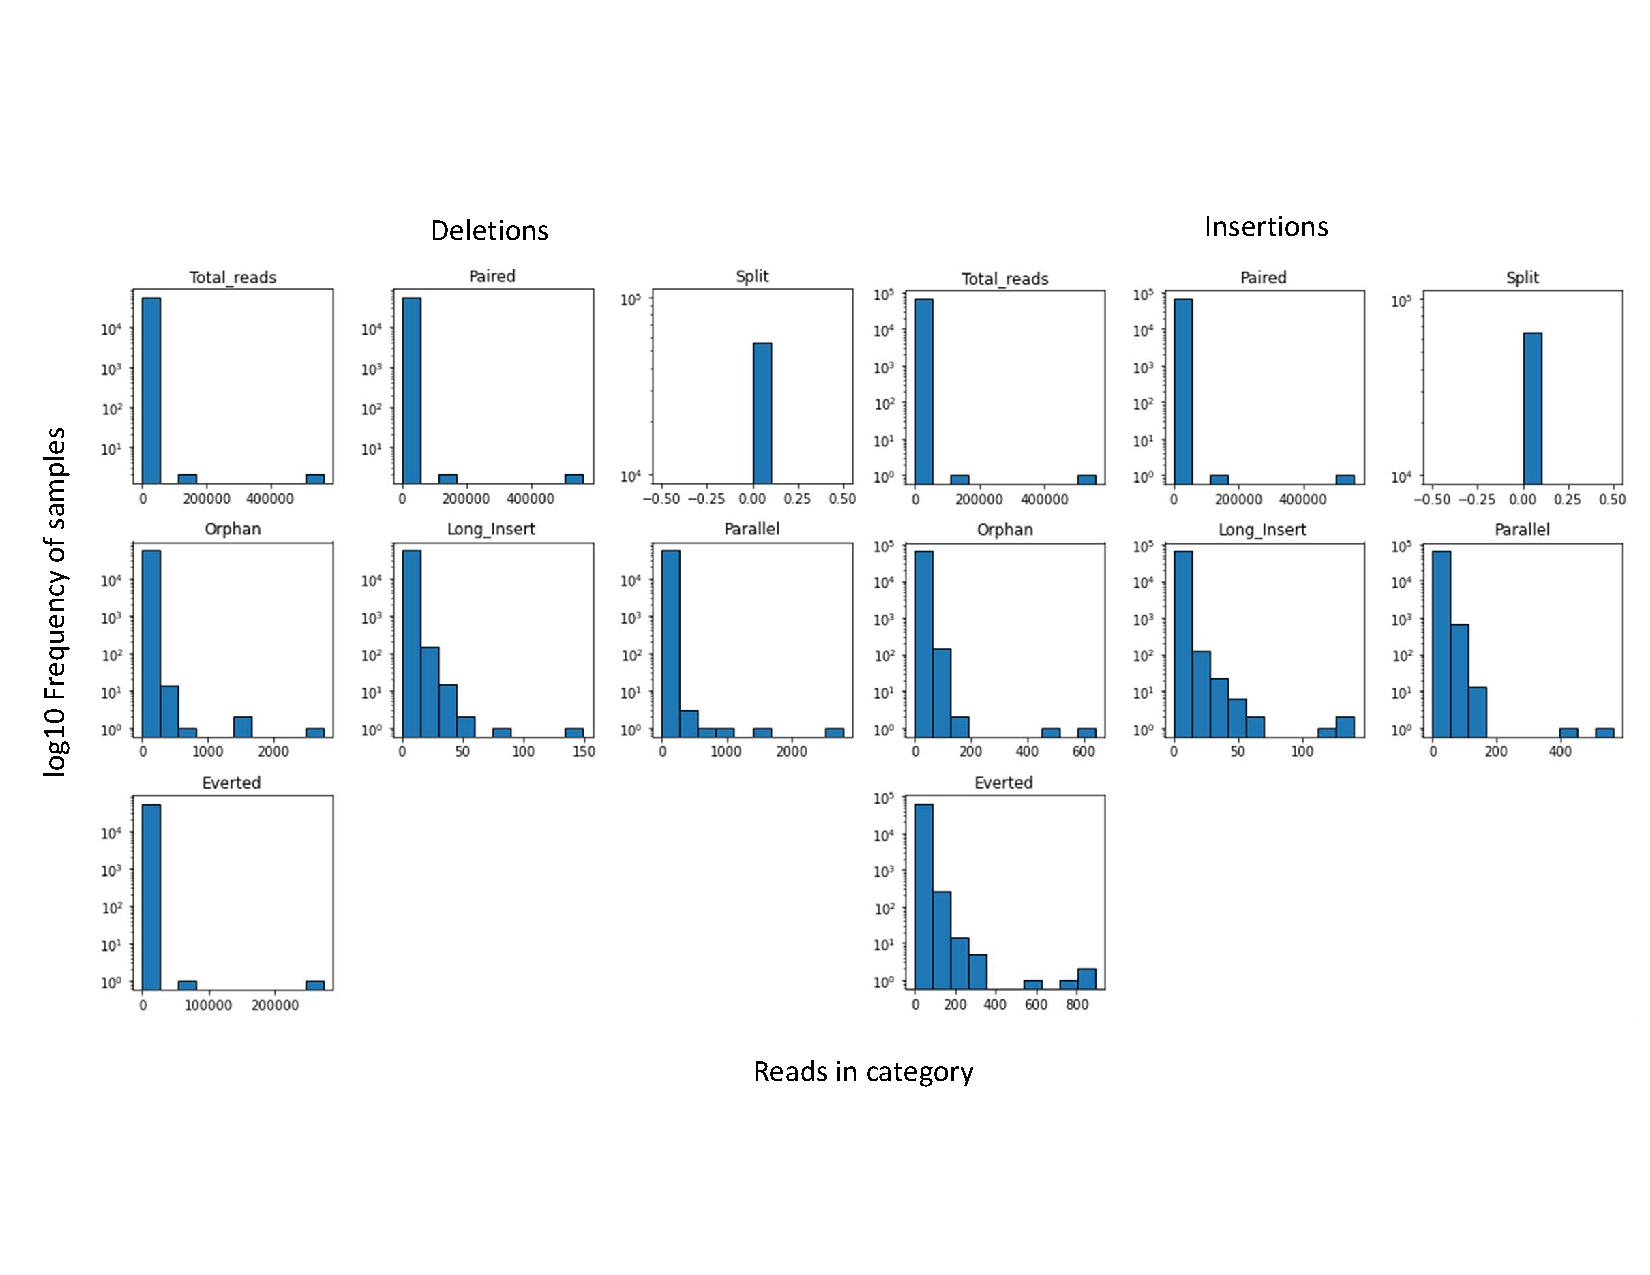
\includegraphics[width=\textwidth]{figures/ch3/read_type_distribution.pdf}}
    \caption[Distribution of read flags per structural variant type.]{Distribution of read flags for insertions and deletions.}
    \label{fig:read-dists}
\end{figure}

\begin{table}[htb]
\resizebox{\textwidth}{!}{%
\begin{tabular}{|l|l|}
\hline
Feature              & Description                                                                                                              \\ \hline
Paired               & Whether the read is single or paired                                                                                     \\ \hline
Proper\_Pair         & Whether the read pair is mapped in the correct order (first read comes before the second in terms of genome coordinates) \\ \hline
Is\_Read1\_Unmapped  & Is the first read unmapped                                                                                               \\ \hline
Is\_Read2\_Unmapped  & Is the second read unmapped                                                                                              \\ \hline
Is\_Read1\_Rev\_Comp & Is the first read reverse complement of the reference                                                                    \\ \hline
Is\_Read2\_Rev\_Comp & Is the second read reverse complement of the reference                                                                   \\ \hline
Is\_First\_Read      & Binary flag for first read                                                                                               \\ \hline
Is\_Second\_Read     & Binary flag for second read                                                                                              \\ \hline
Split                & Is the read non-contiguous (suggesting an insertion within the read itself)                                              \\ \hline
Long\_Insert         & Is the gap between the read pair larger than the 99th percentile of insert lengths across the alignment                  \\ \hline
Short\_Insert        & Is the gap between the read pair smaller than the 2nd percentile of insert lengths across the alignment                  \\ \hline
Parallel\_Read       & Do both reads of the read pair align to the same orientation of the genome                                               \\ \hline
Everted\_Read        & Are the reads in the pair facing away from each other as opposed to towards each other                                   \\ \hline
Orphan\_Read         & Is this read flagged as paired end but the pair does not align to the reference                                          \\ \hline
\end{tabular}%
}

\caption{List of features included in short-read alignment feature respresentation and their description.}

\end{table}

\subsection{Data retrieval and preprocessing}

Data for this study was collected from \textit{Drosophila melanogaster} assemblies and sequencing runs as reported in \cite{chakrabortyEvolutionGenomeStructure2021,chakrabortyHiddenGeneticVariation2018,chakrabortyStructuralVariantsExhibit2019}. In total fourteen \textit{de novo} genome assemblies and associated structural variation callsets (detected using SVMU as described in \cite{chakrabortyStructuralVariantsExhibit2019}) were downloaded. Using the genomic coordinates obtained from the SVMU calls we prepared feature vector representations for all deletions (a segment larger than 50bp is absent compared to the reference), insertions (a segment larger than 50bp is inserted that is not present in the reference), copy number variants (defined here as any duplication), and inversions (a segment inverted along the 5' to 3' orientation as compared to the reference) as well as control regions (regions with no validated structural variant present) using the representation as described above \cite{chakrabortyHiddenGeneticVariation2018}. We then separated out one of the assemblies and callsets to serve as a hold-out test set for all analyses, hereby named the "true test set".

\subsection{Random forest classifier training}

We implemented all random forest classifiers in scikit-learn with the default 500 estimators. For the SV genotyping task the output classes were control (no SV present, a randomly selected region of the genome), deletion, insertion, copy number variant (CNV), and inversion, all of which had a minimum length of 50bp and following the same definition as reported in \cite{chakrabortyEvolutionGenomeStructure2021, chakrabortyHiddenGeneticVariation2018}. Training data was split into a 77\%/33\% train/test split stratified by class labels for equal distribution between the sets. The random forest was fit to the resulting training data and validated on the test data before being applied to hold-out true test set.

\subsection{Copy Number Variant simulation and detection}

We used dudeML \cite{hillDeepLearningApproach2019} to simulate samples with a random number of copies between 2 and 10 with characteristics generated from regions sampled from the test assembly. We then trained a random forest classifier with the number of copies treated as a categorical variable. We split the simulated dataset as 70/30\% training/testing, stratified by class (copy number). This is a separate experiment from the other SV classification tasks, solely to see if we can do downstream prediction on other features of any SVs found such as the number of copies.

\subsection{Object detection model and breakpoint identification}

To detect where SVs and their breakpoints occur in a callset we attempted to use an object detection model (https://github.com/ultralytics/yolov5). This is a form of convolutional neural network that draws boundary boxes and classifies each candidate box, allowing for precise identification of an object and its location within an image. The data representation for object detection is similar to that described in Data retrieval and preprocessing, however instead of summing features as summaries we instead represented each feature as a histogram count of the feature, with the minimum and maximum values of each being standardized across the target region. An example feature map for this data type can be seen in Figure \ref{fig:example_pileup}. 

We attempted two variants of object detection: detecting the entire SV (or in the case of an image not capturing the entire SV, what is present), and identifying breakpoints. In the case of whole-SV detection breakpoints were treated as the left and right bounds for the bounding box values and the entire height of the image was used as the vertical bounds. Bounding box values were scaled relative to 0-1 as described in the YOLOv5 tutorial based on the length of the genomic region represented scaled to a consistent image size of 640 $\times$ 640 pixels. For breakpoint detection we used a 50bp window centered on the identified breakpoint as the left and right bounds, and used the entire y-axis consistent with the entire SV approach. Both were trained under default settings for the YOLOv5s model for 3 epochs.

\begin{figure}
    \centering
    \makebox[\textwidth][c]{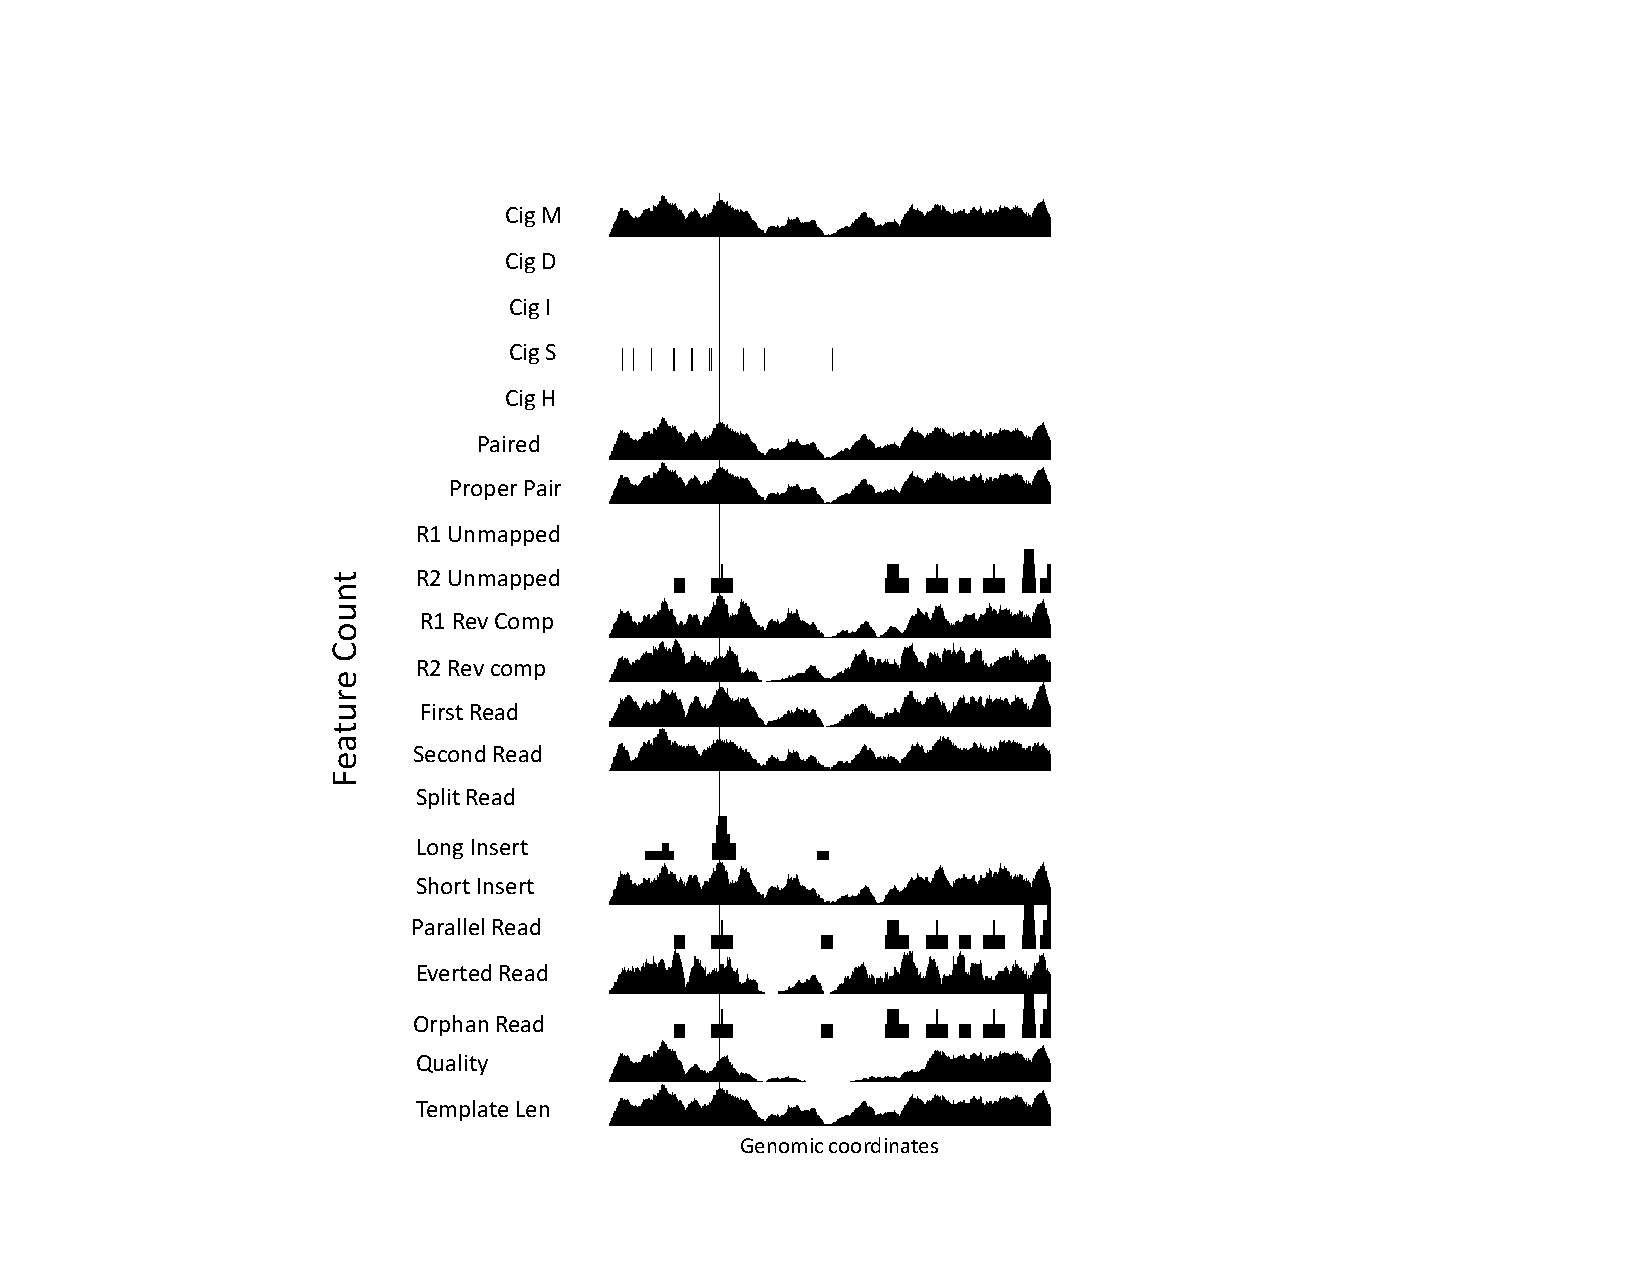
\includegraphics[width=1.5\textwidth]{figures/ch3/example_pileup.pdf}}
    \caption[Sample representations of the object detection feature matrix.]{An example of the object detection feature matrix for a deletion. Grey vertical lines represent the left and right breakpoints for a candidate SV region. "Cig" is an abbreviation for CIGAR string from the SAM file format.}
    \label{fig:example_pileup}
\end{figure}

\subsection{Synthetic transposable element heterozygote creation}
We created a set of synthetic heterozygote transposable element callsets by combining reads of known homozygous reference/alternate genomes. Regions are identified and fastq entries are concatenated, then normalized down to 30x coverage to replicate a true heterozygote sample as in the empirical data. These combined genomes are effectively heterozygous at differing sites, and homozygous at sites which are ref/alt for both assemblies.

\subsection{Transposable element read extraction}

Transposable element (TE) candidate regions are identified by querying fastq sequences for consensus sequences matching to characterized TEs in the reference genome using bedtools. Reads from the candidate genomes are then aligned to this consensus sequence fasta, extracting the names of all reads mapping to a known TE family consensus sequence. These reads are then mapped back to the reference genome for manual inspection using IGV, resulting in a TE-read specific BAM file. 

Ranges in the TE-specific alignment file were then queried for coverage to identify presence of reads in target locations. Ranges that overlap with a reference TE or are not located in euchromatin are filtered out, as well as  regions that are the same length as the average read length. All remaining regions are then expanded by 400bp in either direction and overlapping regions are collapsed, resulting in retained regions with discontinous coverage. 

\subsection{TE breakpoint detection}

The candidate-associated alignments are then queried for soft-clipped reads in the region. To identify breakpoints we first identify all reads with soft-clipped ends >10bp in size and calculate where the starting position of the break is relative to the reported start coordinate of the read. The sites with the highest number of soft-clipped reads aligned to them are reported as breakpoints, assumed in this case to have a target strand duplication, resulting in two breakpoints.

\subsection{Training of TE random forest}

Random forests were trained using 6 synthetic heterozygous genomes (see above) created from the DSPR dataset \cite{chakrabortyStructuralVariantsExhibit2019}. All sequencing runs had a read size of 54bp post-trimming and had a final coverage of 30x. The random forest was trained on chromosomes 3L, 3R, and X, and tested on 2L and 2R, with 500 estimators.

\subsection{McClintock TE callers}

TE calls for competing method benchmarks were obtained by using the McClintock meta-pipeline (found at https://github.com/bergmanlab/mcclintock, v2.0.0) according to instructions for each method.

\section{Results}

\subsection{Summarized features and random forests are a powerful method for SV classification}

To test whether our data representation of summarized features combined with a random forest could accurately identify and distinguish SV types we trained on a large number of long-read validated samples of structural variants in \textit{Drosophila melanogaster}. This long-read data was matched with short-read sequencing data from the same \textit{D. melanogaster} lines that were used to generate feature representations from reference alignments, resulting in a training and testing set for benchmarking multiple methods on SV discovery and characterization. We find that a random forest trained on our summarized data representation achieves high levels of accuracy across multiple SV types on the true test set (Figure \ref{fig:test_accuracy_forest}). One recognized caveat with this approach is the lack of substantial sample numbers for copy number variants and inversions compared to insertions and deletions, and an overall drastic imbalance of all SV types compared to control regions. This is due to three major factors; the first being that structural variants are relatively rare, and while they can span large regions of the genome, the overall composition of a given genome will largely be unaffected (control) regions. The second is that copy number variants in this instance refer to multiple duplication events, however it is possible that some CNVs are treated as insertions, this is largely a semantic difference and will change depending on how the dataset is labeled. And the final caveat is that inversions are extremely rare, so they are expected to be the lowest-represented class in any given SV dataset. Multiple of these issues could be alleviated with simulated SV data, allowing for a more balanced dataset and better representation of different SV types assuming the simulated examples accurately mimic the empirical SVs. 

\begin{figure}
    \centering
    \makebox[\textwidth][c]{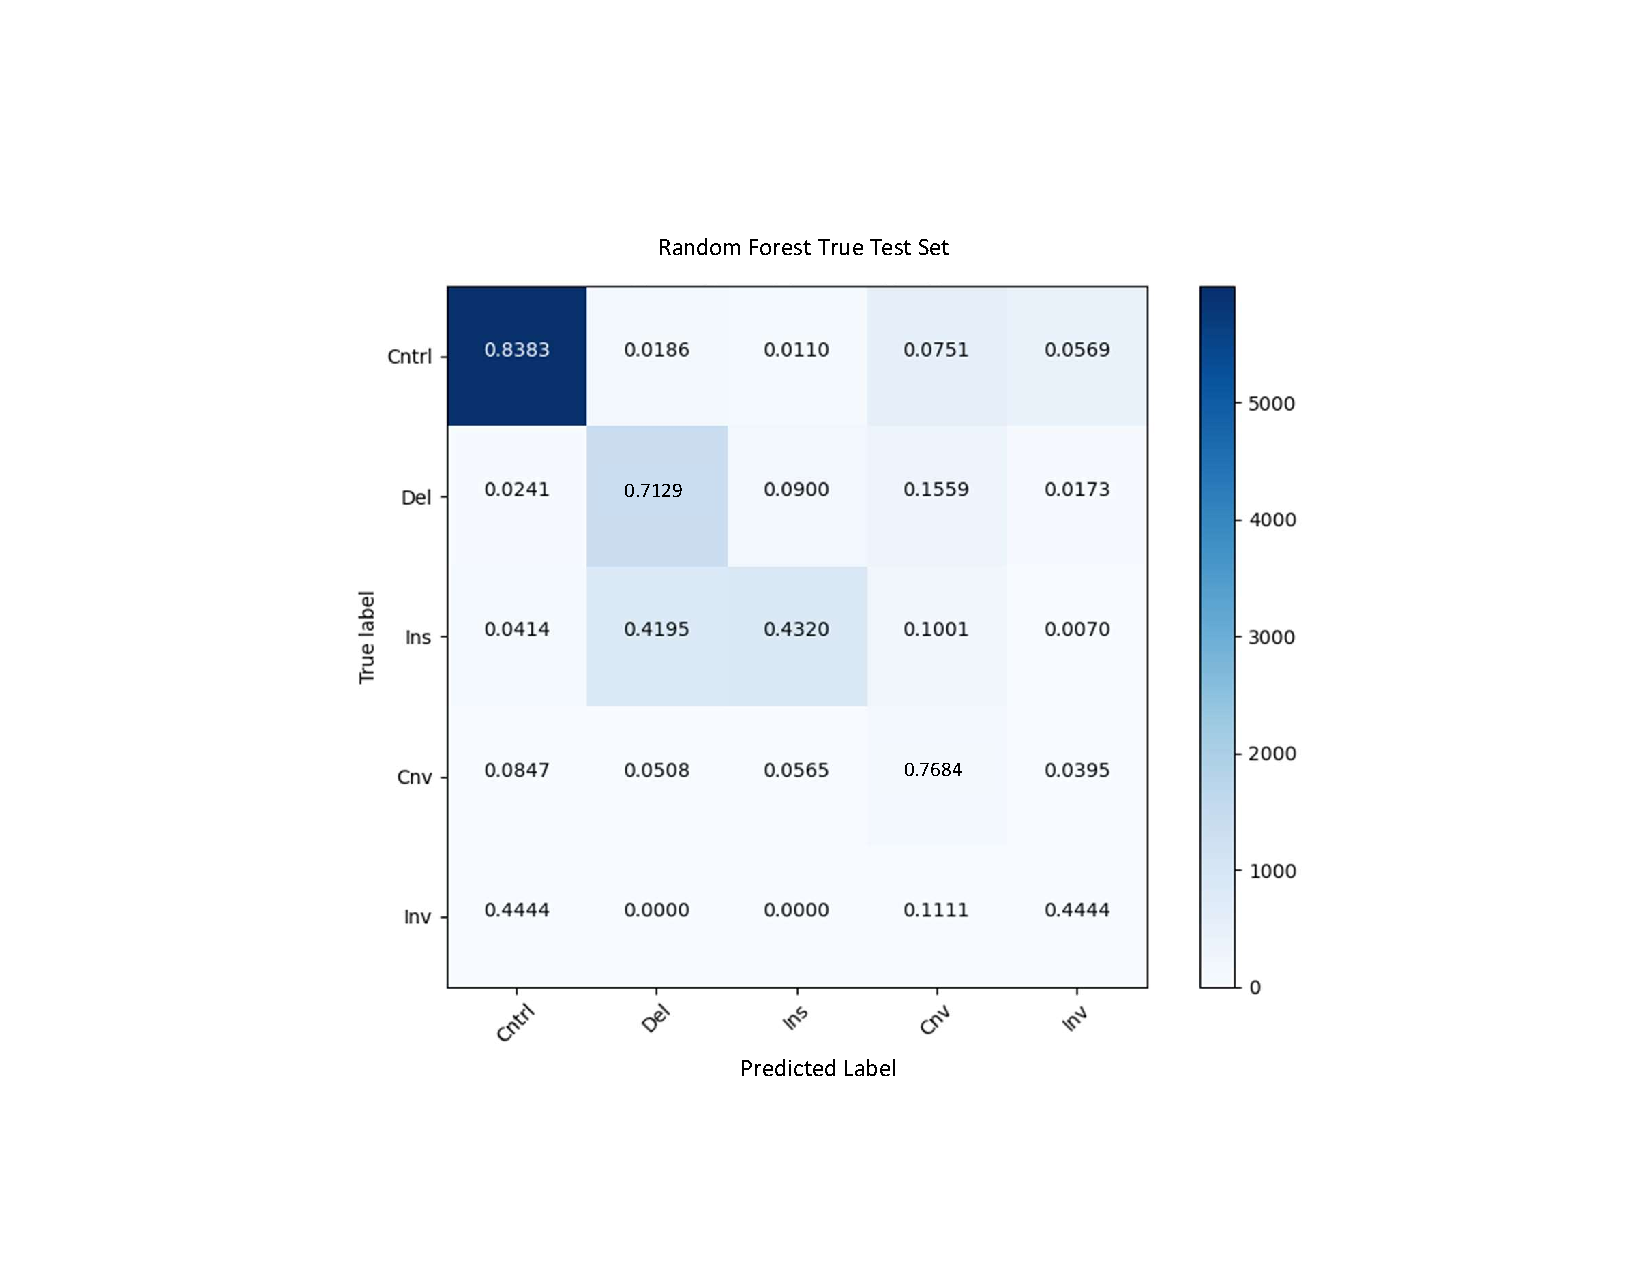
\includegraphics[width=1.5\textwidth]{figures/ch3/test_accuracy_forest.pdf}}
    \caption[Accuracy of random forest on classifying SVs on true test set.]{Accuracy of random forest on classifying SVs on true test set. Labels are controls, deletion, insertions, copy number variants, and inversions, respectively. Values are reported as proportion of true labels (along the y-axis) that are included in a given intersection. Color indicates number of samples in a given intersection scaled to the largest number of samples in a class.}
    \label{fig:test_accuracy_forest}
\end{figure}


\subsection{Random forests provide accuracy boosts when used as a filtering mechanism}

We then tested whether our random forest classifier could be used as a filtering mechanism in tandem with other short-read SV callers. We tested accuracies with and without a modified LastZ \cite{chakrabortyStructuralVariantsExhibit2019} reported candidate SVs in the true test set along with varying softmax thresholds for output probabilities counting as a positive call (Figure \ref{fig:test_accuracy_forest}). LastZ was used here for reporting candidate SVs by comparing alignments of the assemblies against the reference genome, resulting in candidate regions that are mismatched between the two; this calling method is exploited similarly in \cite{chakrabortyEvolutionGenomeStructure2021}. For the non-candidate examples windows of 2,500bp with 1,200bp overlap step size were extracting across the entire genome and predicted on. For LastZ candidate filtering a no-thresholding approach (any class membership posterior probability prediction by the random forest larger than 0.2, 1/5 classes) yields the optimal tradeoff between false positive and true negative rates (Figure \ref{fig:caller_comparison}). Overall performance is vastly improved by using a pre-filtering approach and treating our random forest model as a genotyper, rather than a discovery method. This is reinforced by comparing performance of our approach to some commonly used SV callers, where we find our method to have a higher precision and recall rate than all other competing methods when using LastZ as a discovery method and the random forest as a genotyper, or a tool to be used after previous candidate region identification has been performed (Figure \ref{fig:svbench}).

\begin{figure}
    \centering
    \makebox[\textwidth][c]{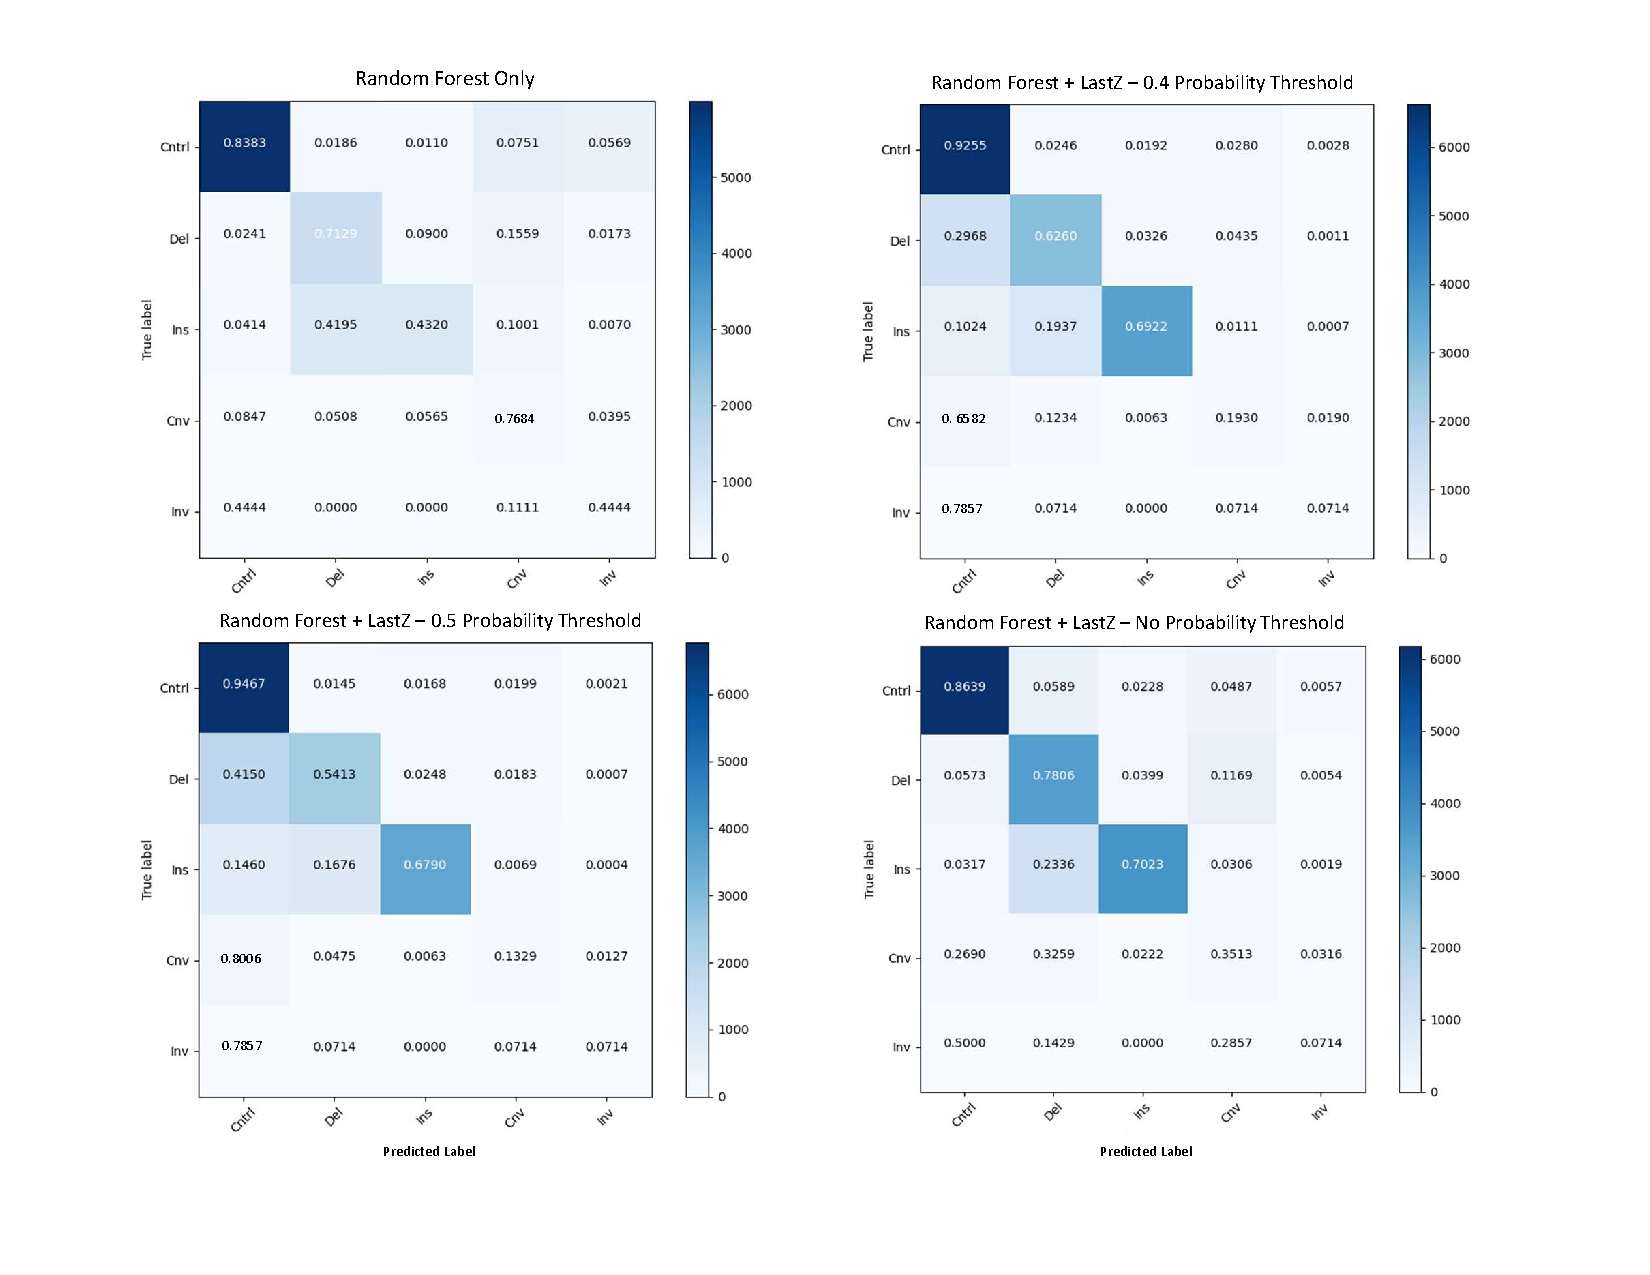
\includegraphics[width=1.2\textwidth]{figures/ch3/thresholding.pdf}}
    \caption[Random Forest caller accuracy with and without prior candidate regions.]{Random Forest caller accuracy with and without prior candidate regions. Probability threshold indicates the probability score cutoff of LastZ that a given candidate site is labelled correctly. Labels are controls, deletion, insertions, copy number variants, and inversions, respectively. Values are reported as proportion of true labels (along the y-axis) that are included in a given intersection. Color indicates number of samples in a given intersection scaled to the largest number of samples in a class.}
    \label{fig:caller_comparison}
\end{figure}

\subsection{Simulated data provides accuracy boosts and out-of-distribution training compared to empirical-only training data}

To test whether our random forest approach could detect more details than presence or absence of SVs we generated a simulated set of CNVs (specifically tandem duplications) using the dudeML package \cite{hillDeepLearningApproach2019}. In brief, a given segment of nucleotides is copied repeatedly adn a label with the amount of times the copy occurs is associated with the segment. Copies can occur in both the forward and reverse orientations, Understanding the number of copies in a duplication can lead to better characterization of its effect on the genome, as dosage-dependent effects are possible with altered copy numbers \cite{fengzhangCopyNumberVariation2009}. We find that this approach is highly effective at identifying copy number in this simulated scenario, demonstrating an accuracy of 89\% across the 5-way classification (Figure \ref{fig:cnvs}). This demonstrates that our feature vector is highly informative at capturing not only the presence of an SV but more detailed information, potentially indicating the ability to characterize other forms of SVs in variant class-specific manners.

\begin{figure}
    \centering
    \makebox[\textwidth][c]{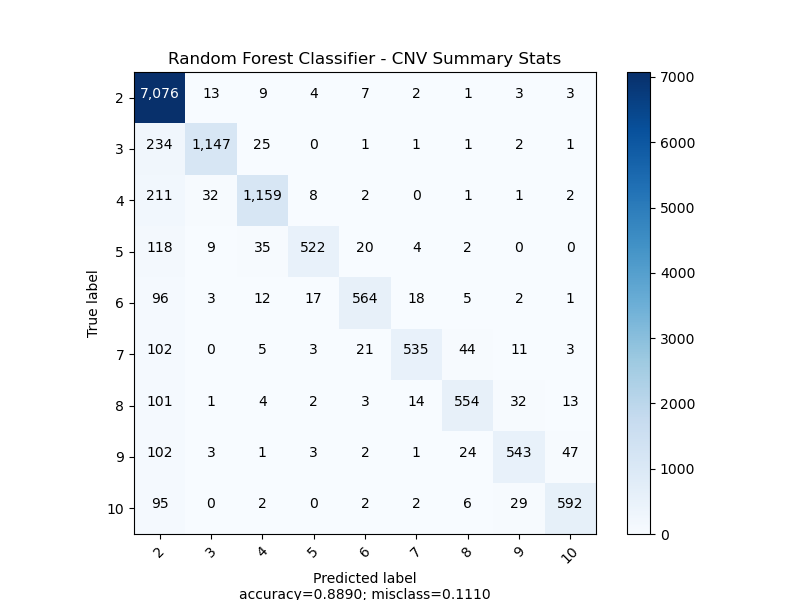
\includegraphics[width=\textwidth]{figures/ch3/Random Forest Classifier - CNV Summary Stats_discriminator_conf_matrix.png}}
    \caption[Random Forest caller accuracy for detecting number of simulated copy numbers.]{Random Forest caller accuracy for detecting number of simulated copy numbers. Simulated CNVs were generated using dudeML and trained/tested on to determine the accuracy of a random forest model for predicting copy number. Values are reported as proportion of true labels (along the y-axis) that are included in a given intersection. Color indicates number of samples in a given intersection scaled to the largest number of samples in a class.}
    \label{fig:cnvs}
\end{figure}


\subsection{SV detection remains a challenging task with object detection frameworks}

We attempted to use an object detection framework (YOLOv5) on an alternative feature vector representation of SVs and their breakpoints. Breakpoint identification is attractive as opposed to whole-SV detection due to its lower computational cost both in terms of creating a feature vector (less genomic information needs to be loaded into memory at any given point when looking for small few-bp breakpoints as opposed to potentially kilobase-scale structural variants).

An additional potential benefit of breakpoint identification is complex SV structures, where a single breakpoint is involved with multiple SV events (a duplication followed by an inversion, for example). Though the whole-SV detection approach allows for an overall easier workflow as no breakpoint matching needs to be done, it is extremely resource intensive, often impossible to fit an entire SV in an "image" with our proposed feature vector (Figure \ref{fig:example_pileup}). We found no significant ability to detect either breakpoints or SVs using this approach (55\% detection accuracy in binary testing for presence of breakpoints), leading us to the conclusion that alternative approaches to either feature engineering, choice of model, or both are necessary to accomplish this task. 

\subsection{Random forests are well suited for detecting transposable elements}

We built a framework for detecting and genotyping the presence of transposable elements (TEs) in the DSPR dataset. As opposed to SVs, TEs have a well-characterized set of consensus sequences that are shared among different types (families) of TEs. These consensus sequences can be exploited to better detect TEs and identify precise breakpoints, a task that has proved much more difficult with SVs. We first generated synthetic heterozygote calls by combining assemblies with known mixtures of TEs and tested all candidate regions for the 2L and 2R chromosomes of a held out test genome. Candidate sites are identified as any region in the reference that contains a TE, this caller is genotyping whether that same TE exists in the target genome at the same location as the reference. We find that the random forest approach is highly effective in this case, demonstrating a high amount of true positive results for the heterozygotes and homozygote TE calls, and notably an extremely high percent of true negative calls (96\% accuracy) despite being run on a large number of candidate sites (Figure \ref{fig:terfconfmat}).

\begin{figure}
    \centering
    \makebox[\textwidth][c]{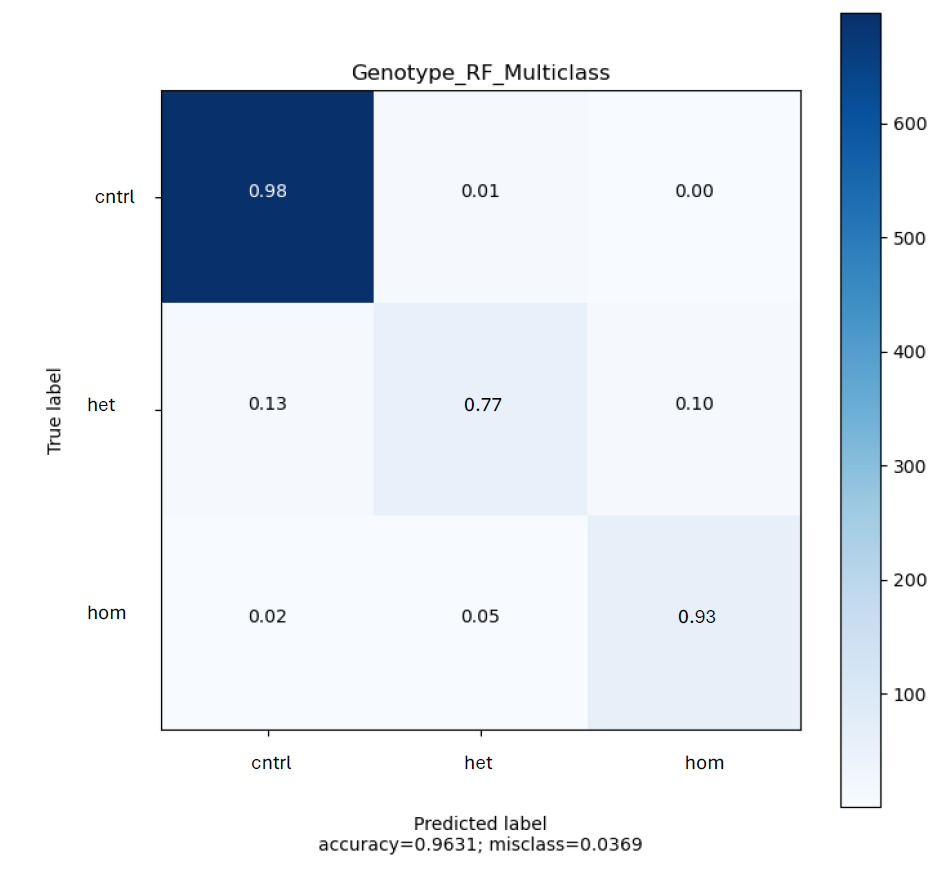
\includegraphics[width=0.8\textwidth]{figures/ch3/cnvrf.png}}
    \caption[Random Forest caller accuracy for detecting presence of TEs.]{Random Forest caller accuracy for detecting presence of TEs. Synthetic TE heterozygote callsets were generated by combining assemblies with known TE presence and location data. Chromosomes 3L, 3R, and X were used for training and 2L and 2R were used for testing.  Values are reported as proportion of true labels (along the y-axis) that are included in a given intersection. Color indicates number of samples in a given intersection scaled to the largest number of samples in a class.}
    \label{fig:terfconfmat}
\end{figure}


To compare our approach to other methods we benchmarked our method (dubbed "TEforest") against a set of commonly used tools for both genotyping including temp and temp2 \cite{yuBenchmarkAlgorithmDetecting2021}, PoPoolationte and PoPoolationte2 \cite{koflerPoPoolation2IdentifyingDifferentiation2011}, teflon \cite{adrionGenomeWideEstimatesTransposable2017}, and retroseq \cite{keaneRetroSeqTransposableElement2013}. The majority of TE discovery and genotyping tools, especially those within the McClintock suite, use some variation of identifying candidate TEs by querying reads in an alignment and using information such as coverage, discordant read pairs, or read clipping as indicators of TE presence. When a certain amount of coverage aligned to a TE consensus sequence, an amount of discordant pair coverage, or some other metric pass a relevant threshold the region is classified as a candidate TE and further validation can occur. This class of method is shown to be highly effective at breakpoint discovery (see Figure S2 for a comparison of our implementation compared to these tools), however genotyping remains a more challenging task. We find that the information present in our alignment feature engineering allows us to outperform other commonly-used TE genotypers, and demonstrates the highest performance across F1 score, precision, and recall on a held out test set (Figure \ref{fig:tebps}) among competitors. We believe this is indicative of two advantages; one being the sheer amount of information in our alignment features and the second being the use of supervised machine learning to provide a model with true positive examples over using heuristics.

\begin{figure}
    \centering
    \makebox[\textwidth][c]{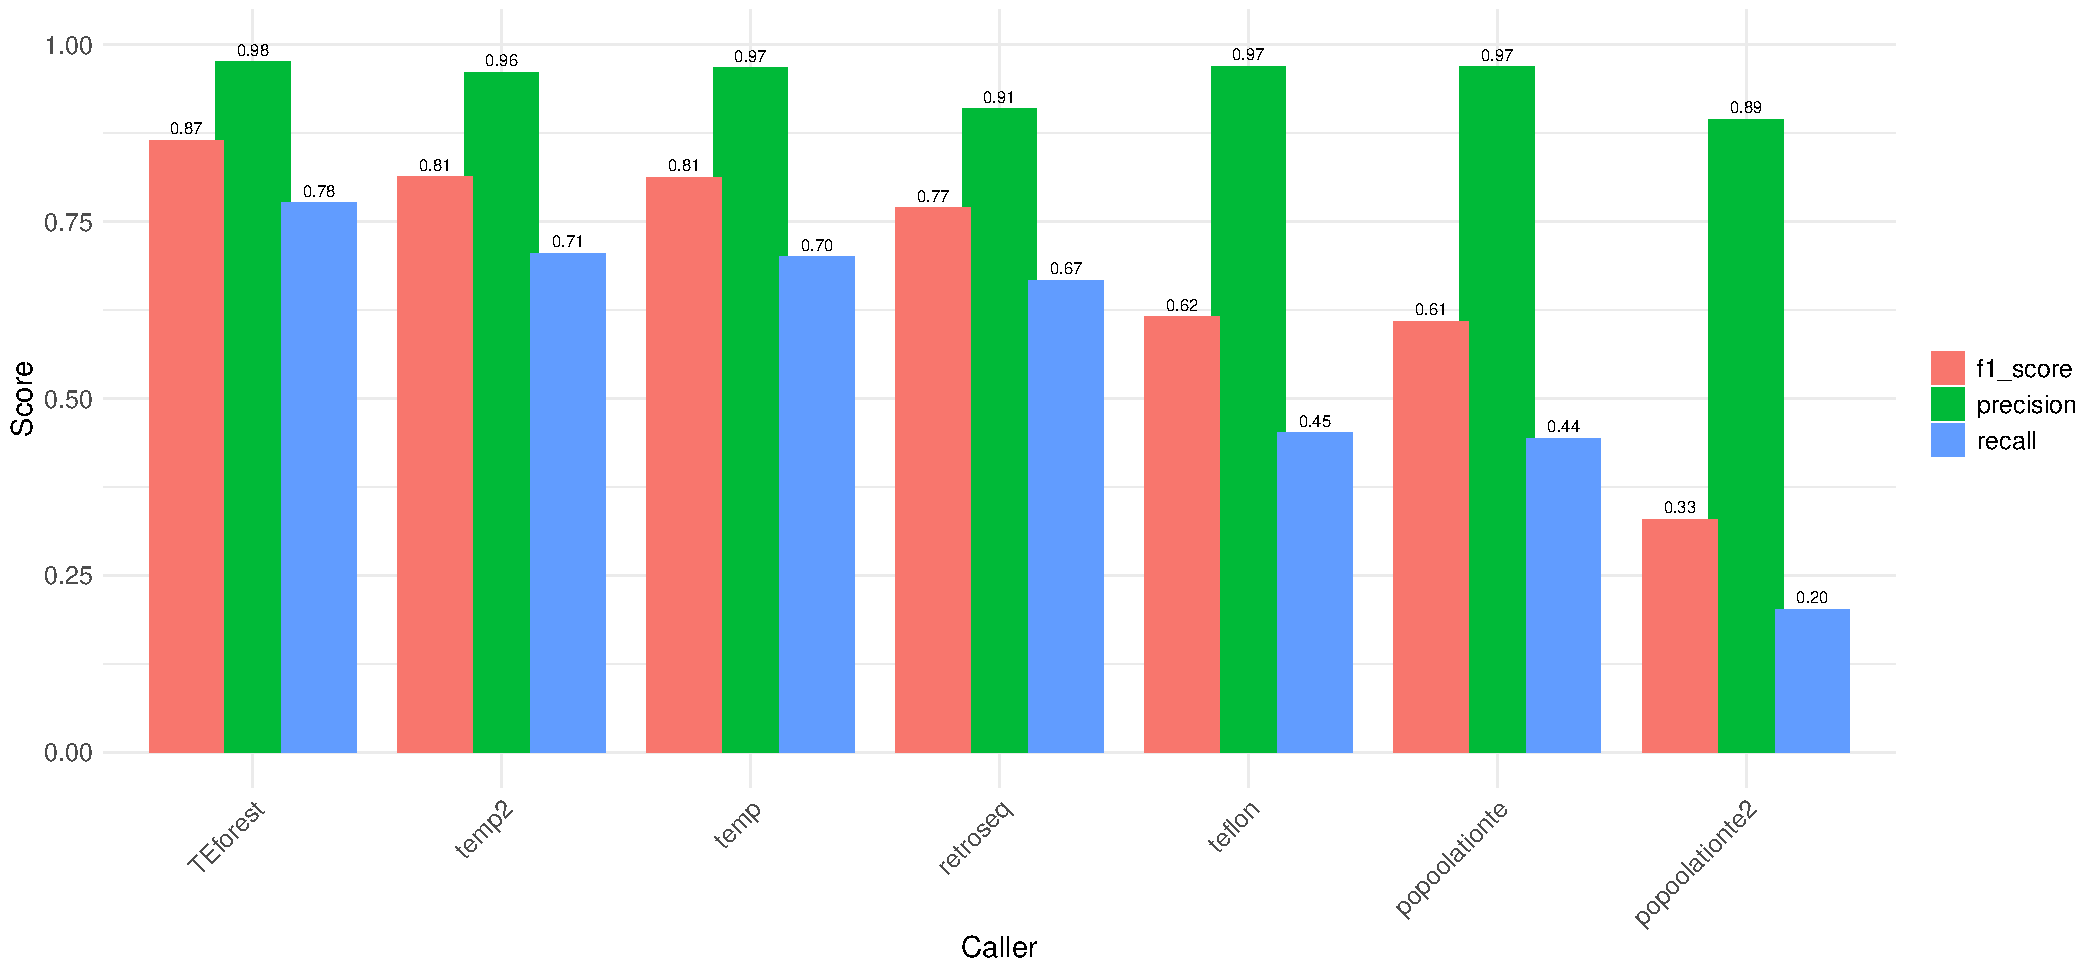
\includegraphics[width=\textwidth]{figures/ch3/performance_forlogan.pdf}}
    \caption[Benchmarking TE genotyping performance between common methods.]{Benchmarking TE genotyping performance between our random forest approach and other common methods. F1 score, precision, and recall are reported for a variety of commonly-used methods.}
    \label{fig:teperf}
\end{figure}

We then tested the ability to detect the presence and location of breakpoints of TEs, as the presence of consensus sequences allows for a heuristic to find candidate TEs and their location in the genome. We developed a method using the soft-clipped segments of read alignments around reference TE sites to detect where more reads than expected contained large numbers of soft-clipped bases and created a region highly likely to be a breakpoint. This candidate breakpoint was then refined to a single base pair coordinate based on the relative end of the clipped bases across all reads covering the candidate region. We find this method to be highly accurate compared to other callers (Figure \ref{fig:svbench}), however it does not achieve state of the art as in the genotyping task.

\section{Discussion}

We attempted to classify and discover structural variants using random forests and state of the art object detection models with a set of long-read and short-read matched sequencing assemblies of \textit{Drosophila melanogaster}. We find that our feature engineering and random forest approach is highly accurate as a filtering mechanism for genotyping candidate SVs, however detection from no prior knowledge or candidates remains a challenging task in the field. Transposable element detection and characterization proved a more feasible task, largely due to the ability to utilize known TE consensus sequences. We found that our approach yielded excellent performance when applied to TE genotyping and breakpoint discovery tasks, leading us to believe there is a path forward in development of this toolset for SV detection and characterization as well.

Structural variants have a large impact on genome function, however our ability to detect them is lagging behind techniques for single nucleotide polymorphisms due to the nature of commonly used short-read sequencing. While long-read sequencing can alleviate some of these issues, there is an enormous amount of existing short-read data available, and short-read remains a cost-effective option for population-scale sequencing. To better characterize structural variant both at the individual and population scale, we believe methods to utilize short-read sequencing are a valuable contribution to the study of genetics.

Despite continuing difficulties with structural variation detection and characterization, we find that our method is extremely capable at detecting and genotyping transposable elements in non-reference samples. This likely stems from the amount of information we include about the alignment in our feature engineering combined with the supervised machine learning approach. Many TE callers filter regions based on mapping quality, orphaned reads, or other information that would typically be filtered in a sequencing analysis workflow \cite{yuBenchmarkAlgorithmDetecting2021} to better match some assumption about what TE-mapped regions should entail, however we utilize this information by making no assumptions about the alignment itself and simply represent the known TEs using all available information. This lack of filtering means we utilize more information but also explicitly train the model on data that would otherwise be unavailable to competing methods, an aspect of this work that is reinforced when observing the feature importance of our model. For example, most of the top features listed in Figure \ref{fig:teshapley} (which is already a subset of the top 10 relevant features by Shapley statistic) are derived from orphan reads, where one read maps to a candidate region and the pair does not map at all. Orphan reads are filtered out by commonly-used methods such as temp2 \cite{yuBenchmarkAlgorithmDetecting2021}. TE insertion sites may be complex, interfering with mapping, but our method trains on real data which allows us to leverage this data and its mapping nuances effectively regardless of this possibility. By training on real data with ground truth annotations these features that are typically filtered out become important for classification rather than a problematic aspect of the alignment to be filtered out. We anticipate further developments in this specific set of tasks and are currently working on developing a more robust breakpoint detection method to match the accuracy demonstrated by our genotyping method.

We propose that with further work into more computationally efficient feature engineering and alternative approaches to object detection our work could be useful in the context of population-scale short-read structural variant calling, allowing for the use of SVs in population genetics analyses where it was previously infeasible.